
\section{Состояние атмосферы}
\begin{frame}{\insertsectionhead}
    \footnotesize
    По информации из ежемесячных отчётов по качеству
    атмосферного воздуха\cite{goveco}, с февраля 2017 года
    по май 2019 года не было выявлено высокого и 
    экстремально высокого загрязнения воздуха.

    \medskip

    По таким примесям, как оксид азота, 
    диоксид серы, аммиак, взвешенные вещества, 
    зафиксированные концентрации были значительно ниже допустимых нормативов
    в указанный период времени. 

    \medskip

    Среднегодовые концентрации оксида азота и формальдегида,
    которые являются токсичными веществами,
    превышают ПДК с.с. по состоянию на 2014-2018 годы.

\end{frame}

\section{Состояние атмосферы \textit{(неофициально)}}
\begin{frame}{\insertsectionhead}
    \begin{minipage}{0.55\textwidth}
        По данным с датчиков тонкодисперсной пыли (PM2.5), 
        установленных неофициально, количество пыли 
        редко превышает 12$\text{мкг}/\text{м}^3$,
        что значительно ниже нормы (35$\text{мкг}/\text{м}^3$).

        \medskip

        Данные в сайта IQAir\cite{iqair} приводят к тем же выводам.
    \end{minipage}
    \begin{minipage}{0.40\textwidth}
        \hspace{1em}
        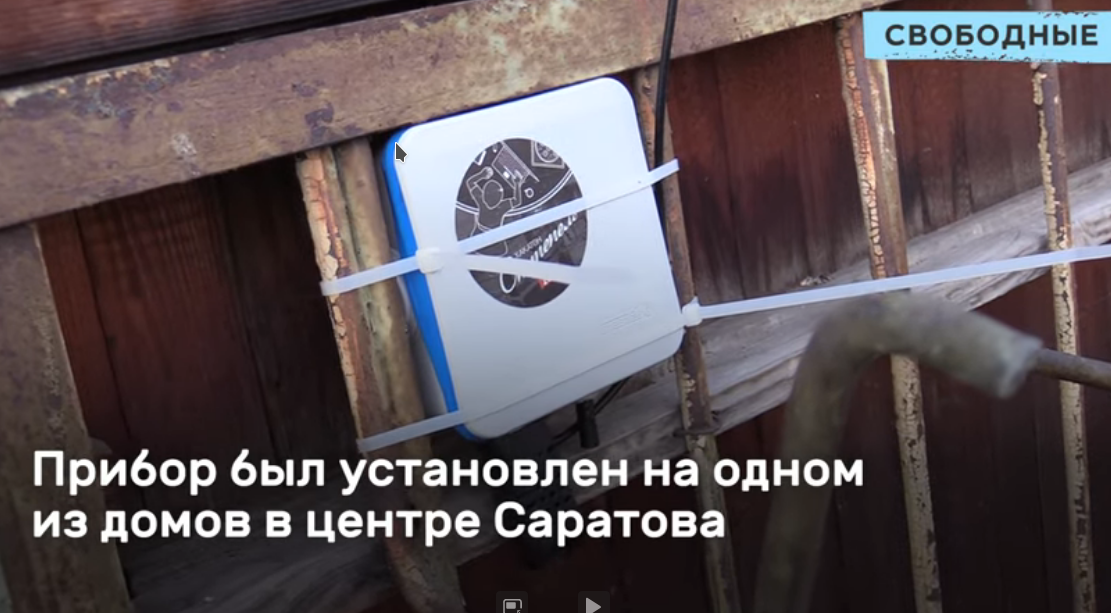
\includegraphics[width=\textwidth]{assets/device.png}
    \end{minipage}
\end{frame}

